%!TEX program = xelatex

\documentclass[compress]{beamer}
%--------------------------------------------------------------------------
% Common packages
%--------------------------------------------------------------------------
\usepackage[english]{babel}
\usepackage{pgfpages} % required for notes on second screen
\usepackage{graphicx}
\usepackage{subfigure}
\usepackage{multicol}

\usepackage{tabularx,ragged2e}
\usepackage{booktabs}

\usepackage{setspace}

%--------------------------------------------------------------------------
% Load theme
%--------------------------------------------------------------------------
\usetheme{hri}

\usepackage{dtklogos} % must be loaded after theme
\usepackage{tikz}
\usetikzlibrary{calc,mindmap,backgrounds,positioning,svg.path}

\graphicspath{{figs/}}

%--------------------------------------------------------------------------
% General presentation settings
%--------------------------------------------------------------------------
\title{Mutual Modelling in Robotics}
\subtitle{Inspiration for the Next Steps}
\date{Human-Robot Interaction, 2015, Portland}
\author{\scriptsize {\Medium Séverin Lemaignan}, Pierre Dillenbourg}
\institute{Computer-Human Interaction\\for Learning and Instruction {\Medium
EPFL}}

%--------------------------------------------------------------------------
% Notes settings
%--------------------------------------------------------------------------
%\setbeameroption{show notes on second screen}
%\setbeameroption{hide notes}

% for mutual modelling
\newcommand{\Mmodel}[3]{{\mathcal{M}(#1, #2, #3)}}
\newcommand{\model}[3]{{$\mathcal{M}(#1, #2, #3)$}}
\newcommand{\Model}[3]{{$\mathcal{M}^{\circ}(#1, #2, #3)$}}


\newsavebox{\ontoinstance}
\savebox{\ontoinstance}{
\begin{tikzpicture}[
    >=latex,
    every edge/.style={<-, draw, very thick},
    every node/.style={draw, font=\sf, node distance=0.5, rounded corners,
    align=center, inner sep=5pt,fill=hriSec2Dark!50},
    classof/.style={<-, draw=black!60, dashed},
    property/.style={<-, draw=hriSec2Comp},
    propname/.style={above, draw=none, fill=none, font=\tt, inner sep=2pt},
    instance/.style={draw=hriSec1Dark, font=\sf, node distance=0.5, rounded corners,
align=center, inner sep=5pt, fill=none}]

    \node[fill=hriSec2Comp!50] (thing) {\textbf{thing}};
    \node [fill=hriSec3CompDark!50, node distance=1.8, below left=of
    thing](sthing) {place} edge[dashed] (thing);
    \node [fill=hriSec3CompDark!50, below left=of sthing] (agent) {agent} edge (sthing);
        \node [fill=hriSec3CompDark!50, below=of sthing] (artifact) {artifact} edge (sthing);
        \node [fill=hriSec3CompDark!50, below right=of sthing] (location) {physical
        support} edge (sthing);
        \node [fill=hriSec3CompDark!50, below right=of artifact] (table) {table}
            edge (location) edge (artifact);


    \node [node distance=1, below right=of thing] (tthing) {temporal thing} edge (thing);
        \node [below right=of tthing] (evt) {event} edge[dashed] (tthing);
                    \node [below right=of evt] (act) {action} edge (evt);

  \draw[dotted, thick] (-5,-5) -- (7.5, -5);

  \node [instance, below=3 of agent] (human) {human\_1} edge[classof, bend left] (agent);
  \node [instance, above right=of human, anchor=south] (robot) {pr2\_robot} edge[classof, bend left] (agent);
  \node [instance, right=of human, anchor=north west] (book) {book\_game\_thrones}
  edge[classof] (artifact);
  \node [instance, right=2 of robot] (ikea) {ikea\_table} edge[classof, bend
  right] (table);
  \node [instance, right=2 of book] (red) {red} edge[property] node[propname] {hasColor} (book);

  \draw[dotted, thick] (-5,-8) -- (7.5, -8);

  \path (book.200) edge [property, out=-100, in=-80, looseness=2]
  node[propname,auto] {isNextTo} (human.south);
  \path (book.270) edge [property, out=-100, in=-90, looseness=3.5] node[propname,auto] {looksAt} (robot.south);
  \path (ikea.south) edge [property, out=-90, in=-80, looseness=3] node[propname, auto] {isOn} (book.320);
\end{tikzpicture}
}


\begin{document}

\begin{frame}{}
\Large

This presentation is made available under a Creative Commons
Attribution-ShareAlike license.

\begin{center}
    \includegraphics[width=0.8\linewidth]{cc-by-sa}
\end{center}

{\Medium EXCEPT} for the Gruffalo pictures that are Copyright Julia Donaldson
and Axel Scheffler.

\end{frame}

\maketitle

\whiteimageframe{sally_ann}

\section{1- A gentle introduction to epistemic modal logic with...}
\imageframe{gruffalo}
\whiteimageframe{gruffalo1}
\whiteimageframe{gruffalo2}
\whiteimageframe{gruffalo3}
\whiteimageframe{gruffalo4}

\begin{frame}{The mouse is an epistemic logician}

$\mathsf{K}$: epistemic operator "{\Medium knows}", $\mathsf{B}$: doxatic operator
"{\Medium believes}"

$m$ stands for the mouse, $f$ for the fox, $g$ for the Gruffalo

$p$ stands for $\exists g$

\Large

\only<1-2>{

\[
\mathsf{K}_{m}\neg p \wedge \mathsf{K}_{m}\neg\mathsf{K}_{f}\neg p 
\]
\uncover<2>{
    \begin{center}
        \includegraphics[width=0.3\linewidth]{gruffalo-fox}
    \end{center}

    \begin{center}
$m$ performs action $\rightarrow \mathsf{B}_{f}p$
    \end{center}
}
}

\only<3-4>{
    \begin{center}
        \includegraphics[width=0.3\linewidth]{gruffalo2}

$p$ stands! 

%    \uncover<4>{
%knowledge revision $\rightarrow \mathsf{K}_{m}p$
%}
    \end{center}
}

\only<5-6>{
\[
    \mathsf{K}_{m}\neg\mathsf{K}_{g}\mathsf{B}_{f}\neg p 
%\uncover<6>{
%    \wedge \mathsf{B}_{g}\mathsf{K}_{f}p
%}
\]
\uncover<6>{
    \begin{center}
        \includegraphics[width=0.3\linewidth]{gruffalo-fox2}
    \end{center}


}
}
%
%\only<7>{
%    \small
%    \begin{enumerate}
%        \item Fox: $\mathsf{K}_{f}p \wedge \mathsf{B}_{f}(areFriends(m,g)) \wedge
%            \mathsf{B}_{f}(wantsToEat(g,f))$
%        \item Gruffalo: $\mathsf{B}_{g}(fears(f,m))$
%    \end{enumerate}
%}


\end{frame}

\imageframe{gruffalo-robot}

%%%%%%%%%%%%%%%%%%%%%%%%%%%%%%%%%%%%%%%%%%%%%%%%%%%%%%%%%%%%%%%%%%%%%%%%%%%%%%%
%%%%%%%%%%%%%%%%%%%%%%%%%%%%%%%%%%%%%%%%%%%%%%%%%%%%%%%%%%%%%%%%%%%%%%%%%%%%%%%
%%%%%%%%%%%%%%%%%%%%%%%%%%%%%%%%%%%%%%%%%%%%%%%%%%%%%%%%%%%%%%%%%%%%%%%%%%%%%%%

\section{$\mathsf{K}_{severin}(\neg funny)$}


\begin{frame}{Shopping list for HRI?}
    \centering
    \begin{tabular}{p{0.5\linewidth}p{0.5\linewidth}}
        \toprule
        {\Medium In the HRI fridge...} & {\Medium To buy...} \\
        \midrule
        Instrumental gestures & Expressive gestures \\
        Using person as tool & Using person as receiver of information \\
        Talking about desires and emotions & Talking about beliefs and ideas \\
        Showing "active" sociability & Showing "interactive" sociability \\
        Elicited structured play & Spontaneous pretend play \\
        \bottomrule
    \end{tabular}
\end{frame}


{ \paper{Frith and Happé, {\Medium Autism: Beyond "theory of
    mind"}, Cognition, 1994}
\begin{frame}{Autistic assets and deficits observed in real life}
    \centering
    \begin{tabular}{p{0.5\linewidth}p{0.5\linewidth}}
        \toprule
        {\Medium Assets} & {\Medium Deficits} \\
        \midrule
        Instrumental gestures & Expressive gestures \\
        Using person as tool & Using person as receiver of information \\
        Talking about desires and emotions & Talking about beliefs and ideas \\
        Showing "active" sociability & Showing "interactive" sociability \\
        Elicited structured play & Spontaneous pretend play \\
        \bottomrule
    \end{tabular}
\end{frame}
}

\section{2- The tasks' zoo}

\whiteimageframe{zoo}

{
    \paper{Baron-Cohen,
        {\Medium Out of sight or out of mind? another
        look at deception in autism}, Journal of Child
    Psychology and Psychiatry, 1992}
\begin{frame}{Object occlusion vs Information occlusion}
    \begin{center}
    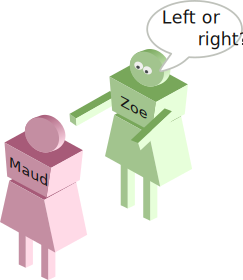
\includegraphics[width=0.6\textwidth]{penny-hiding-game.pdf}
    \end{center}

\end{frame}
}


{
    \paper{Wimmer and Perner, {\Medium Beliefs about beliefs:
    Representation and constraining function [...]}, Cognition, 1983}
\begin{frame}{1st order ToM: the False-Belief Experiment}

    \begin{center}
    \only<1>{
    \includegraphics[width=0.7\textwidth]{sally_ann.pdf}
    }
    \only<2>{
    \includegraphics[width=0.6\textwidth]{triadic_false_beliefs.pdf}\\
    (hello Bilge!)
    }
    \end{center}
\end{frame}
}


{
    \paper{Flobbe, Verbrugge, Hendriks, Krämer,
        {\Medium Children's application of theory of mind in reasoning
    and language}, Journal of Logic, Language and
    Information, 2008}
\begin{frame}{2nd order ToM: the Chocolate Bar Experiment}
    \begin{center}
    \includegraphics[width=0.65\textwidth]{chocolate-bar.pdf}
    \end{center}

\end{frame}
}

{
    \paper{Verbrugge, {\Medium Logic and social cognition}, Journal of Philosophical
    Logic, 2009}
\begin{frame}{Agreement as $\infty$-order ToM}
    \only<1>{
    \begin{center}
    \includegraphics[width=0.4\textwidth]{mutual-agreement.pdf}
    \end{center}
}
\only<2->{
    \begin{center}
    \includegraphics[width=0.2\textwidth]{mutual-agreement.pdf}
    \end{center}

    \uncover<2->{
    Shared knowledge
\[
    \mathsf{EK}_J\varphi \leftrightarrow \bigwedge_{i \in J}\mathsf{K}_i\varphi
\]
}
\uncover<3>{
    Common knowledge 
\[
    \mathsf{CK}_J\varphi \leftrightarrow
\mathsf{EK}_J\varphi \wedge \mathsf{EK}_J\mathsf{EK}_J\varphi \wedge
\mathsf{EK}_J\mathsf{EK}_J\mathsf{EK}_J\varphi \wedge ...
\]
}
}
\end{frame}
}

\section{3- Triangles, rectangles}

\begin{frame}{}
    \only<1>{
        \begin{multicols}{2}

            \includegraphics[width=0.9\columnwidth]{triadic_false_beliefs.pdf}

            \columnbreak

            \mbox{}\vfill

            \begin{itemize}
                \item \model{A}{B}{X}
                \item \Model{A}{B}{X}
            \end{itemize}

            \scriptsize
            e.g. {\color{hriSec1} \model{\text{robot}}{\text{Sally}}{plans}}

            \vfill\mbox{}

        \end{multicols}
    }

    \only<2>{
        \begin{multicols}{2}
            \vspace*{0.4cm}
            \includegraphics[width=0.9\columnwidth]{triadic_false_beliefs.pdf}



            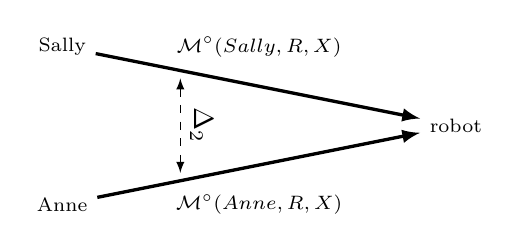
\begin{tikzpicture}[
                    >=latex,
                scale=0.5]

                \draw(0,2) node (A) {\scriptsize Sally};
                \draw(0,-2) node (B) {\scriptsize Anne};
                \draw(10,0) node (C) {\scriptsize robot};

                \draw(5,2) node {\scriptsize \Model{Sally}{ R}{ X}};
                \draw(5,-2) node {\scriptsize \Model{Anne}{ R}{ X}};
                \draw[dashed, <->] (3,1.2) -- (3,-1.2) node[midway, sloped, above] {$\Delta_2$};
                \draw[->,very thick] (A) to (C);
                \draw[->,very thick] (B) to (C);

            \end{tikzpicture}

            \vspace*{1cm}

            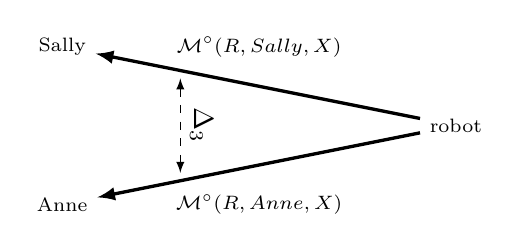
\begin{tikzpicture}[
                    >=latex,
                scale=0.5]

                \draw(0,2) node (A) {\scriptsize Sally};
                \draw(0,-2) node (B) {\scriptsize Anne};
                \draw(10,0) node (C) {\scriptsize robot};

                \draw(5,2) node {\scriptsize \Model{R}{ Sally}{ X}};
                \draw(5,-2) node {\scriptsize \Model{R}{ Anne}{ X}};
                \draw[dashed, <->] (3,1.2) -- (3,-1.2) node[midway, sloped, above]
                {$\Delta_3$};
                \draw[<-,very thick] (A) to (C);
                \draw[<-,very thick] (B) to (C);

            \end{tikzpicture}
        \end{multicols}
    }
    \only<3>{
        Do Sally and Anne have the same accuracy when modelling the robot?

        {\centering
            \(\Delta_2 = \Delta(\Mmodel{\text{Sally}}{R}{X}, \Mmodel{\text{Anne}}{R}{X})\)

        }

        \vspace*{1em}
        Conversely, what may lead the robot to model more accurately
        Sally or Anne?

        {\centering
            \(\Delta_3= \Delta(\Mmodel{R}{\text{Sally}}{X},
            \Mmodel{R}{\text{Anne}}{X})\)

        }

    }
\end{frame}

\begin{frame}{}

    \begin{multicols}{2}
        \vspace*{0.6cm}
        \begin{center}
        \includegraphics[width=0.6\columnwidth]{robot_false_beliefs.pdf}
        \end{center}

        \vspace*{1.3cm}
        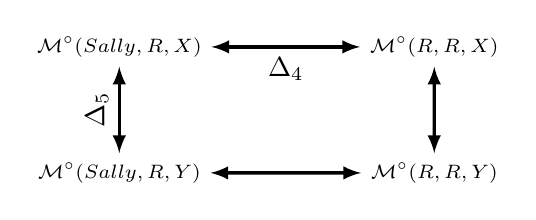
\begin{tikzpicture}[>=latex, scale=0.4]

            \draw(0,0) node (a) {\scriptsize \Model{Sally}{R}{ X}};
            \draw(10,0) node (b) {\scriptsize \Model{R}{R}{ X}};
            \draw(10,-4) node (c) {\scriptsize \Model{R}{R}{ Y}};
            \draw(0,-4) node (d) {\scriptsize \Model{Sally}{R}{ Y}};
            \draw[<->,very thick] (a) -- (b) node[midway, below] {$\Delta_4$};
            \draw[<->,very thick] (b) -- (c);
            \draw[<->,very thick] (c) -- (d);
            \draw[<->,very thick] (d) -- (a) node[midway, sloped, above] {$\Delta_5$};

        \end{tikzpicture}
    \end{multicols}



\end{frame}

\section{Alright, take home message}

\begin{frame}{Take home message}
    \begin{center}
    \uncover<1->{Read the litterature on autism in developmental psychology (and
        if only one paper, Frith and Happé's one): it certainly resonnates to
    roboticists' ears \\[1em]}
    \uncover<2->{The models found in CSCL raise practical questions that we may
    want to research too \\[1em]}
    \uncover<3->{Even if deep learning is all hype, modal logics
        bring useful formal models to the table (and bridges to philosophy of mind as
    bonus). We should give them another look.}

        \end{center}
\end{frame}

\imageframe[{\Medium Thank you!}\\ severin.lemaignan@epfl.ch]{gruffalo2}
%
%\section{Today's standards}
%
%\begin{frame}{}
%    \begin{itemize}
%        \item Scassellati,
%        \item Alami,
%        \item Trafton with ACT-R/E
%        \item Breazeal,
%        \item Belpaeme,
%        \item ...
%
%    \end{itemize}
%\end{frame}
%
%{
%\paper{Lemaignan, Alami, {\Medium Explicit Knowledge and the Deliberative Layer: Lessons Learned}, IROS 2013}
%\begin{frame}{One Instantiation}
%
%    \begin{center}
%        \uncover<2->{
%        \includegraphics[width=0.9\textwidth]{spark.pdf}
%    }
%
%    \begin{multicols}{2}
%        \centering
%        \includegraphics[width=\columnwidth]{pr2-scene.jpg}
%        
%        \begin{figure}
%
%        \resizebox{\columnwidth}{!}{%
%        \begin{tikzpicture}[
%            yscale=1.3,
%            >=latex,
%            every edge/.style={<-, draw, very thick},
%            every node/.style={draw, font=\sf, node distance=0.5, rounded corners,
%            align=center, inner sep=5pt,fill=hriSec2Dark!50},
%            classof/.style={<-, draw=black!60, dashed},
%            property/.style={<-, draw=hriSec2Comp},
%            propname/.style={above, draw=none, fill=none, font=\tt, inner sep=2pt},
%            instance/.style={draw=hriSec1Dark, font=\sf, node distance=0.5, rounded corners,
%        align=center, inner sep=5pt, fill=none}]
%
%            \node[fill=hriSec2Comp!50] (thing) {\textbf{thing}};
%            \node [fill=hriSec3CompDark!50, node distance=1.8, below left=of
%            thing](sthing) {place} edge[dashed] (thing);
%            \node [fill=hriSec3CompDark!50, below left=of sthing] (agent) {agent} edge (sthing);
%                \node [fill=hriSec3CompDark!50, below=of sthing] (artifact) {artifact} edge (sthing);
%                \node [fill=hriSec3CompDark!50, below right=of sthing] (location) {physical
%                support} edge (sthing);
%                \node [fill=hriSec3CompDark!50, below right=of artifact] (table) {table}
%                    edge (location) edge (artifact);
%
%
%            \node [node distance=1, below right=of thing] (tthing) {temporal thing} edge (thing);
%                \node [below right=of tthing] (evt) {event} edge[dashed] (tthing);
%                            \node [below right=of evt] (act) {action} edge (evt);
%
%        \uncover<3->{
%        \draw[dotted, thick] (-5,-3.8) -- +(13, 0);
%
%        \node [instance, below=3 of agent] (human) {baby\_1} edge[classof, bend left] (agent);
%        \node [instance, above right=of human, anchor=south] (robot) {pr2\_robot} edge[classof, bend left] (agent);
%        \node [instance, right=of human, anchor=north west] (book) {book\_game\_thrones}
%        edge[classof] (artifact);
%        \node [instance, right=2 of robot] (ikea) {ikea\_table} edge[classof, bend
%        right] (table);
%        \node [instance, right=2 of book] (brown) {brown} edge[property] node[propname] {hasColor} (book);
%
%
%        %}
%        %\uncover<3>{
%        \draw[dotted, thick] (-5,-6.2) -- +(13, 0);
%
%        \node [instance, below=5 of act] (moving) {move\_act\_42} edge[classof] (act);
%        \path (moving.west) edge [property, out=180, in=-80, looseness=1] node[propname,below] {currentlyPerforms} (human.230);
%
%        \path (human.280) edge [property, out=-80, in=-90, looseness=3.5] node[propname,right] {looksAt} (robot.south);
%        \path (ikea.south) edge [property, out=-90, in=-80, looseness=3] node[propname, auto] {isOn} (book.320);
%        }
%        \end{tikzpicture}
%        }
%
%        \end{figure}
%
%    \end{multicols}
%
%    \end{center}
%\end{frame}
%
%\imageframe{humans-pt}
%
%{
%\paper{Ros et al., {\Medium Which One? Grounding the Referent Based on Efficient HRI}, ROMAN 2010}
%\begin{frame}{One Model per Agent}
%        \begin{multicols}{2}
%            \begin{figure}
%                \resizebox{0.35\textwidth}{!}{\usebox{\ontoinstance}}
%            \end{figure}
%            \begin{figure}
%                \resizebox{0.35\textwidth}{!}{\usebox{\ontoinstance}}
%            \end{figure}
%            \begin{figure}
%                \resizebox{0.35\textwidth}{!}{\usebox{\ontoinstance}}
%            \end{figure}
%            {\vspace*{1.5cm}\hspace*{2.5cm}\huge...}
%        \end{multicols}
%\end{frame}
%}
%

\end{document}






